\section{Held-out Results}
\IfFileExists{generated/main_results_matrix.tex}{\begin{table*}[t]
\centering\footnotesize
\caption{Held-out FLORES+ devtest results (1{,}012 items per direction; all planned outputs, including baseline fallback). C: COMET-22$\times$100; $\Delta$: post-edit minus sentence-split NLLB (S0) with paired 95\% bootstrap interval; markers use Holm-adjusted $p$ over the 24-test primary family ($^\dagger p<.05$, $^\ddagger p<.01$). FB: baseline fallbacks. BLEU/chrF++ are descriptive.}
\label{tab:main}
\setlength{\tabcolsep}{3pt}
\resizebox{\textwidth}{!}{%
\begin{tabular}{llrrrrrrrrrrrr}
\toprule
 & & \multicolumn{3}{c}{En$\to$Tl} & \multicolumn{3}{c}{Tl$\to$En} & \multicolumn{3}{c}{En$\to$Es} & \multicolumn{3}{c}{Es$\to$En} \\
\cmidrule(lr){3-5}\cmidrule(lr){6-8}\cmidrule(lr){9-11}\cmidrule(lr){12-14}
Editor & Strategy & C & $\Delta$ [95\% CI] & FB & C & $\Delta$ [95\% CI] & FB & C & $\Delta$ [95\% CI] & FB & C & $\Delta$ [95\% CI] & FB \\
\midrule
\multicolumn{2}{l}{S0 split NLLB} & 85.20 & -- & -- & 87.57 & -- & -- & 86.67 & -- & -- & 87.37 & -- & -- \\
\midrule
GPT-4o Mini & Zero & 85.84 & +0.64$^\ddagger$ [+0.50, +0.77] & 0 & 88.39 & +0.83$^\ddagger$ [+0.69, +0.97] & 0 & 86.95 & +0.28$^\ddagger$ [+0.17, +0.39] & 0 & 87.71 & +0.34$^\ddagger$ [+0.24, +0.46] & 0 \\
 & One & 86.15 & +0.95$^\ddagger$ [+0.78, +1.12] & 0 & 88.57 & +1.00$^\ddagger$ [+0.83, +1.18] & 0 & 87.20 & +0.53$^\ddagger$ [+0.37, +0.69] & 0 & 87.73 & +0.36$^\ddagger$ [+0.24, +0.50] & 0 \\
 & Reason & 85.71 & +0.51$^\ddagger$ [+0.38, +0.64] & 0 & 88.22 & +0.65$^\ddagger$ [+0.50, +0.81] & 0 & 86.93 & +0.26$^\ddagger$ [+0.14, +0.38] & 0 & 87.64 & +0.27$^\ddagger$ [+0.17, +0.39] & 0 \\
\midrule
Llama 3 8B & Zero & 84.72 & -0.48$^\ddagger$ [-0.65, -0.32] & 0 & 87.47 & -0.10 [-0.26, +0.05] & 0 & 86.68 & +0.00 [-0.18, +0.19] & 0 & 87.36 & -0.01 [-0.13, +0.12] & 0 \\
 & One & 84.81 & -0.39$^\ddagger$ [-0.57, -0.21] & 0 & 87.60 & +0.03 [-0.12, +0.18] & 0 & 86.85 & +0.18 [-0.05, +0.40] & 0 & 87.33 & -0.04 [-0.24, +0.16] & 0 \\
 & Reason & 83.76 & -1.44$^\ddagger$ [-1.70, -1.21] & 0 & 86.25 & -1.32$^\ddagger$ [-1.57, -1.07] & 0 & 86.16 & -0.51$^\ddagger$ [-0.71, -0.31] & 0 & 86.63 & -0.74$^\ddagger$ [-0.93, -0.55] & 0 \\
\bottomrule
\end{tabular}}
\end{table*}
}{\begin{table*}[t]
\centering\footnotesize
\caption{Held-out FLORES+ devtest results (1{,}012 items per direction; all planned outputs, including baseline fallback). \pending{placeholder layout --- this table is generated by Phase 5 into generated/main\_results\_matrix.tex}}
\label{tab:main}
\setlength{\tabcolsep}{3pt}
\resizebox{\textwidth}{!}{%
\begin{tabular}{llrrrrrrrrrrrr}
\toprule
 & & \multicolumn{3}{c}{En$\to$Tl} & \multicolumn{3}{c}{Tl$\to$En} & \multicolumn{3}{c}{En$\to$Es} & \multicolumn{3}{c}{Es$\to$En} \\
\cmidrule(lr){3-5}\cmidrule(lr){6-8}\cmidrule(lr){9-11}\cmidrule(lr){12-14}
Editor & Strategy & C & $\Delta$ [95\% CI] & FB & C & $\Delta$ [95\% CI] & FB & C & $\Delta$ [95\% CI] & FB & C & $\Delta$ [95\% CI] & FB \\
\midrule
\multicolumn{2}{l}{S0 split NLLB} & 00.00 & -- & -- & 00.00 & -- & -- & 00.00 & -- & -- & 00.00 & -- & -- \\
\midrule
GPT-4o Mini & Zero & 00.00 & +0.00 [+0.00, +0.00] & 0 & 00.00 & +0.00 [+0.00, +0.00] & 0 & 00.00 & +0.00 [+0.00, +0.00] & 0 & 00.00 & +0.00 [+0.00, +0.00] & 0 \\
 & One & 00.00 & +0.00 [+0.00, +0.00] & 0 & 00.00 & +0.00 [+0.00, +0.00] & 0 & 00.00 & +0.00 [+0.00, +0.00] & 0 & 00.00 & +0.00 [+0.00, +0.00] & 0 \\
 & Reason & 00.00 & +0.00 [+0.00, +0.00] & 0 & 00.00 & +0.00 [+0.00, +0.00] & 0 & 00.00 & +0.00 [+0.00, +0.00] & 0 & 00.00 & +0.00 [+0.00, +0.00] & 0 \\
\midrule
Llama 3 8B & Zero & 00.00 & +0.00 [+0.00, +0.00] & 0 & 00.00 & +0.00 [+0.00, +0.00] & 0 & 00.00 & +0.00 [+0.00, +0.00] & 0 & 00.00 & +0.00 [+0.00, +0.00] & 0 \\
 & One & 00.00 & +0.00 [+0.00, +0.00] & 0 & 00.00 & +0.00 [+0.00, +0.00] & 0 & 00.00 & +0.00 [+0.00, +0.00] & 0 & 00.00 & +0.00 [+0.00, +0.00] & 0 \\
 & Reason & 00.00 & +0.00 [+0.00, +0.00] & 0 & 00.00 & +0.00 [+0.00, +0.00] & 0 & 00.00 & +0.00 [+0.00, +0.00] & 0 & 00.00 & +0.00 [+0.00, +0.00] & 0 \\
\bottomrule
\end{tabular}}
\end{table*}
}
Results follow the research questions, after the overall comparison with S0. All 24 conditions contain the planned 1{,}012 items per direction, and every output passed the output contract: no condition used the baseline fallback (Table~\ref{tab:main}). The measured effects are therefore editing behaviour, not contract failure. As a diagnostic outside the test families, sentence splitting itself raised S0 above the unsplit system by $+0.39$ (En$\to$Tl), $+0.21$ (En$\to$Es), and $+0.08$ points (Tl$\to$En); Es$\to$En was inconclusive.

\textbf{Overall effect against S0 (F1).} GPT-4o Mini improves on S0 in every direction and strategy, by +0.26 to +1.00 points, all significant after Holm correction; five of these intervals, all in the Spanish pair, lie within $\pm0.5$ points, so several gains are clear but small. Llama 3 8B never improves significantly. Its zero-shot and one-shot outputs are significantly worse only for En$\to$Tl ($\DLlamathreeEightZeroShotEngTag$ and $\DLlamathreeEightKnnOneshotEngTag$), with the other six intervals inside $\pm0.5$ points, and reason-then-edit is significantly worse in all four directions ($\DLlamathreeEightReasonThenEditEngSpa$ to $\DLlamathreeEightReasonThenEditEngTag$). BLEU and chrF++ lie above S0 for all twelve GPT-4o Mini conditions and below it for all twelve Llama conditions, including those where COMET does not change significantly.

\textbf{RQ1: pairs and baseline quality.} GPT-4o Mini gains are larger for the Tagalog pair (+0.51 to +1.00) than for the Spanish pair (+0.26 to +0.53), and Llama losses are also largest for Tagalog. The Tagalog directions, however, contain more weak drafts (S0 COMET $<0.80$: 183 and 82 items, against 104 and 60). Within this improve pool, GPT-4o Mini one-shot gains are similar across pairs (+3.11 to +5.29 points), while in the protect pool (S0 $\geq0.90$) every GPT-4o Mini condition stays near zero ($-0.16$ to $+0.15$). Baseline quality explains only part of the pair difference, however: reweighting each direction to the pooled weak/middle/strong mix narrows GPT-4o Mini's Tagalog--Spanish gap by 16--23\%, and at least 73\% of the remaining gap arises in mid-quality drafts (exploratory).

\textbf{RQ2: strategies (F2).} \NsigStrategy{} of 24 strategy contrasts are significant after Holm correction. For GPT-4o Mini, the retrieved exemplar beats zero-shot in three directions (+0.17 to +0.31; Es$\to$En inconclusive), and reason-then-edit falls below one-shot in the same three ($-0.27$ to $-0.44$) but below zero-shot only for Tl$\to$En ($-0.18$). For Llama, one-shot and zero-shot do not differ significantly in any direction, whereas reason-then-edit is significantly worse than both in all four ($-0.51$ to $-1.35$).

\IfFileExists{figures/fig_bands.pdf}{\begin{figure}[t]\centering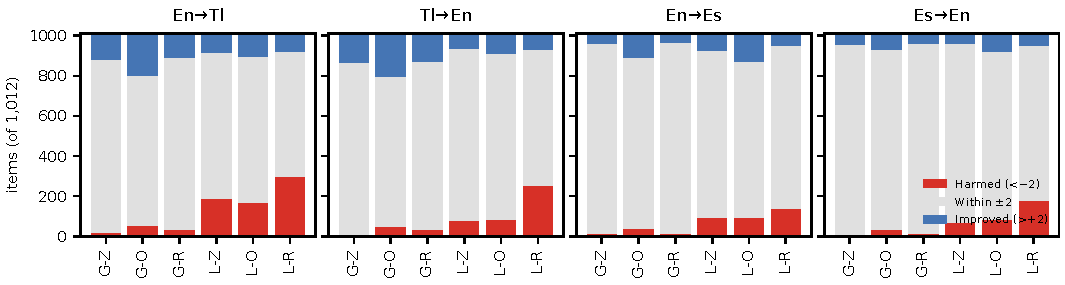
\includegraphics[width=\columnwidth]{figures/fig_bands.pdf}\caption{Improved ($>$+2 points), within-band, and harmed ($<-$2) devtest items per condition (G/L: GPT-4o Mini/Llama; Z/O/R: zero-shot/one-shot/reason-then-edit). Unchanged outputs lie within the band.}\label{fig:bands}\end{figure}}{}
\IfFileExists{generated/overediting_table.tex}{\begin{table}[t]
\centering\footnotesize
\caption{Protect-pool over-editing on devtest: over-edited items / protect-pool items per direction (protect: S0 COMET$\geq$0.90; over-edit: text changed and native COMET loss $>$0.02).}
\label{tab:overedit}
\setlength{\tabcolsep}{3pt}
\begin{tabular}{llrrrr}
\toprule
Editor & Strategy & En$\to$Tl & Tl$\to$En & En$\to$Es & Es$\to$En \\
\midrule
GPT-4o Mini & Zero & 3/234 & 3/377 & 3/275 & 1/293 \\
 & One & 6/234 & 26/377 & 7/275 & 12/293 \\
 & Reason & 5/234 & 13/377 & 3/275 & 4/293 \\
\midrule
Llama 3 8B & Zero & 42/234 & 35/377 & 29/275 & 26/293 \\
 & One & 35/234 & 37/377 & 28/275 & 33/293 \\
 & Reason & 57/234 & 107/377 & 32/275 & 51/293 \\
\bottomrule
\end{tabular}
\end{table}
}{}
\textbf{RQ3: over-editing of strong drafts.} Edit rate alone does not predict harm (Fig.~\ref{fig:bands}, Table~\ref{tab:overedit}). GPT-4o Mini one-shot changes 3{,}249 of 4{,}048 drafts (80\%) yet over-edits only 51 of 1{,}179 strong drafts (4.3\%); its zero-shot and reason-then-edit rates are 0.8\% and 2.1\%. Llama edits at similar rates but over-edits 11.2\% (zero-shot), 11.3\% (one-shot), and 20.9\% (reason-then-edit), up to 107 of 377 strong Tl$\to$En drafts. Llama harms more segments than it improves in 9 of 12 conditions; GPT-4o Mini improves more than it harms in all 12.

\textbf{RQ4: direction.} Direction effects are small and inconsistent: GPT-4o Mini gains more into English than out of English for every strategy in the Tagalog pair (e.g., $\DGptfourMiniZeroShotTagEng$ vs.\ $\DGptfourMiniZeroShotEngTag$ zero-shot), but not in the Spanish pair (one-shot $\DGptfourMiniKnnOneshotSpaEng$ into English vs.\ $\DGptfourMiniKnnOneshotEngSpa$ out of English).

\textbf{Robustness (exploratory).} No F1 decision changes under Bonferroni or Benjamini--Hochberg correction, or under Holm over both families jointly, and all 18 significant F1 effects have the same sign in COMET, BLEU, and chrF++. Wilson 95\% intervals keep the pooled over-editing rates apart (GPT-4o Mini at most 5.6\%, Llama at least 9.5\%), and among edited drafts every GPT-4o Mini condition harms at most 8.9\% of them, below the 9.9\% minimum for Llama.

\textbf{Summary.} GPT-4o Mini improved every condition and rarely damaged strong drafts; Llama improved none. The retrieved exemplar helped GPT-4o Mini most, and reason-then-edit ranked last for both editors in every direction.
